\section{ 1: Ethernet simulation}
In this question, we are going to simulate Ethernet using a hub and a switch and investigate the performance of the network under different conditions. For this question, you can get help from the examples in the directory ``inet4.5/examples/ethernet/lans''.
\subsection{part 1}
\begin{enumerate}
    \item In this part, we are going to simulate a simple star-topology network. As shown in Figure 2, one \texttt{EthernetHub} module and 8 \texttt{EthernetHost} modules are used. Use \texttt{Eth10M} for the channel and set length parameter to 10m. You can find these modules in \texttt{inet.node.ethernet} package. Assume one of the hosts as a server(sending no traffic) and others as clients. Run simulation for 50 sec. Set the other parameters as follows:
    \begin{itemize}
        \item \texttt{**.cli.sendInterval = exponential(100ms)}
        \item \texttt{**.cli.reqLength = intuniform(50,1400)*1B}
        \item \texttt{**.cli.respLength = intWithUnit(truncnormal(3000B,3000B))}
    \end{itemize}
    
    In the results folder of your project, you should be able to find a \texttt{.sca} file. Double-click on it to create a \texttt{.anf} file. Then, go to the `Browse Data' tab in the \texttt{.anf} file, select the `Scalers' tab, and collect the following statistics to include in your report: \texttt{rx channel idle(\%)}, \texttt{rx channel utilization(\%)}, \texttt{rx channel collision(\%)} for each host. Further, calculate \textit{network throughput(bit/sec)} = \textit{total number of bits successfully arrived} / \textit{simulation time}. To do so, you can use \texttt{packetReceived:sum(packetBytes)} in the statistics.
\end{enumerate}
\begin{qsolve}
    \begin{qsolve}[]
        thi .ini file and .ned file are shown in figure 1 and 2. for the ned file it is a simple network with parts from inet framework.in ini file i just set the destination of host1 to null so it doesnt send any packets as client and set other hosts destination to host 1 so they send their data to host 1 and it acts as a server. the results are as below:
        \begin{enumerate}
            \item \texttt{rx channel idle(\%)} shown in figure 3
            \item \texttt{rx channel utilization(\%)} shown in figure 4
            \item \texttt{rx channel collision(\%)} shown in figure 5
            \item \texttt{packetReceived:sum(packetBytes)} shown in figure 6
        \end{enumerate}
        \splitqsolve[\splitqsolve]
        \begin{figure}[H]
            \centering
            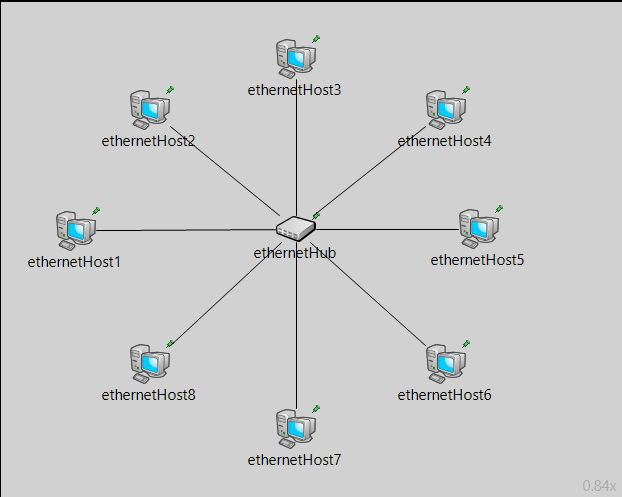
\includegraphics[width=0.8\textwidth]{Q1_1ned.png}
            \caption{network for Q1 part 1}
        \end{figure}
        \begin{figure}[H]
            \centering
            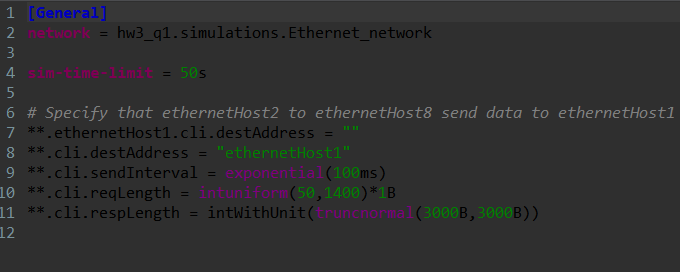
\includegraphics[width=0.8\textwidth]{Q1_1ini.png}
            \caption{ini file for Q1 part 1}
        \end{figure}
        \begin{figure}[H]
            \centering
            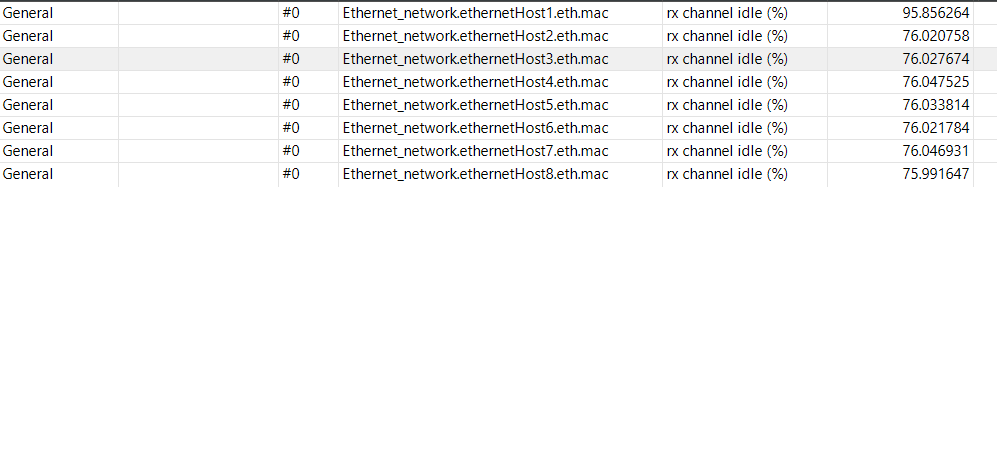
\includegraphics[width=0.75\textwidth]{output1.png}
            \caption{rx channel idle(\%) for Q1 part 1}
        \end{figure}
        \splitqsolve[\splitqsolve]
        \begin{figure}[H]
            \centering
            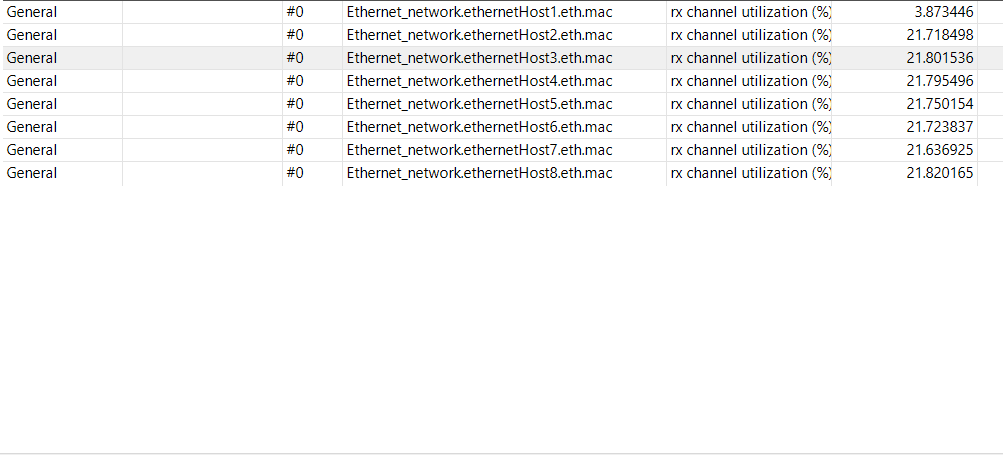
\includegraphics[width=0.8\textwidth]{output2.png}
            \caption{rx channel utilization(\%) for Q1 part 1}
        \end{figure}
        \begin{figure}[H]
            \centering
            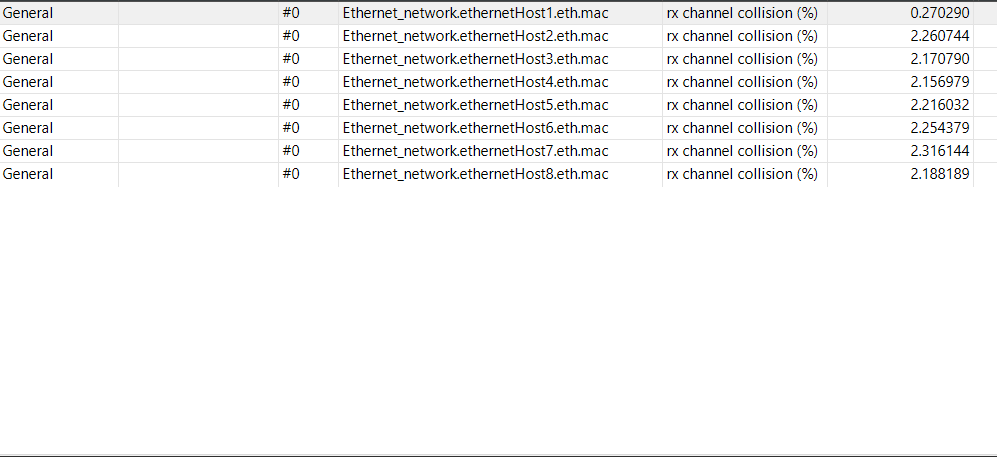
\includegraphics[width=0.8\textwidth]{output3.png}
            \caption{rx channel collision(\%) for Q1 part 1}
        \end{figure}
        \begin{figure}[H]
            \centering
            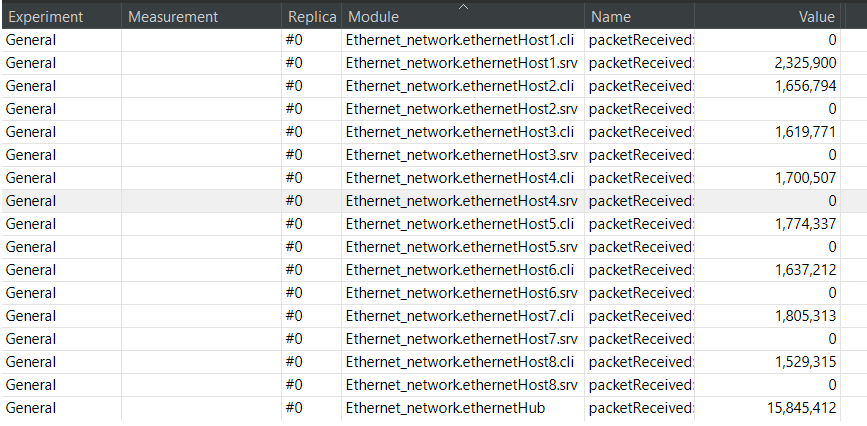
\includegraphics[width=0.8\textwidth]{output4.png}
            \caption{packetReceived:sum(packetBytes) for Q1 part 1}
        \end{figure}
        so the network throughput is $\frac{11723249\times 8\ bits}{50\ s} \simeq 1.872 Mbps$
    \end{qsolve}
\end{qsolve}
\subsection{part 2}
Replace the \texttt{EthernetHost} module with the \texttt{EthernetSwitch} module. Repeat Part 1 for this new network configuration (other configuration setups are the same as part 1). Compare the collision rate and network throughput with those from Part 1 and explain the results. Additionally, include the MAC address table of the switch in your report.
\begin{qsolve}
    \begin{qsolve}[]
        the ini file is as the same as part 1 but the ned file is changed to use switch instead of host the network is shown in figure 7. the results are as below:
        \begin{enumerate}
            \item \texttt{rx channel idle(\%)} shown in figure 8
            \item \texttt{rx channel utilization(\%)} shown in figure 9
            \item \texttt{rx channel collision(\%)} shown in figure 10
            \item \texttt{packetReceived:sum(packetBytes)} shown in figure 11
            \item \texttt{MAC address table} shown in figure 12
        \end{enumerate}
        \begin{figure}[H]
            \centering
            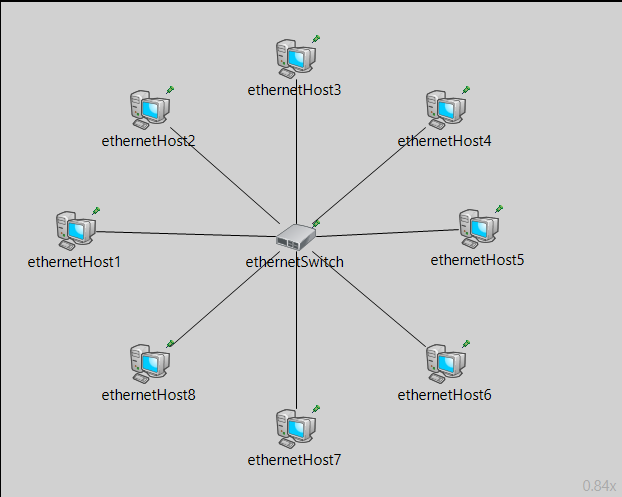
\includegraphics[width=0.7\textwidth]{Q1_2ned.png}
            \caption{network for Q1 part 2}
        \end{figure}
        \begin{figure}[H]
            \centering
            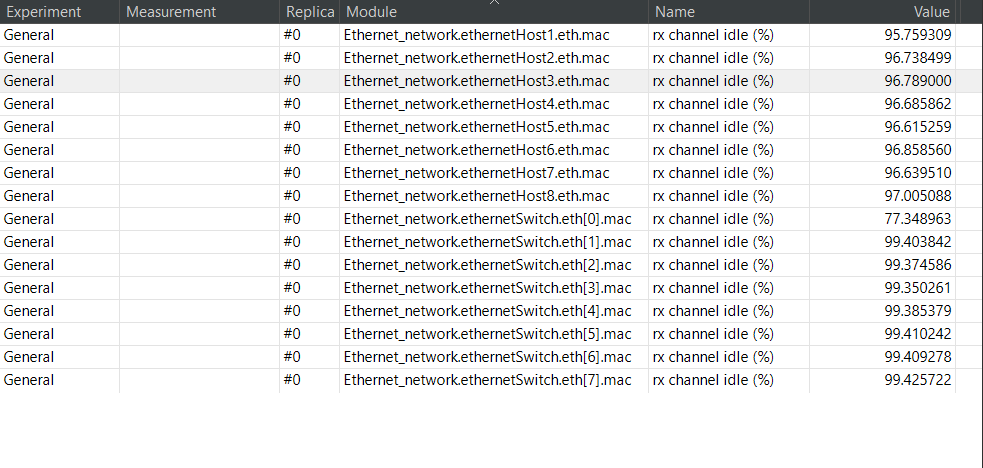
\includegraphics[width=0.7\textwidth]{output5.png}
            \caption{rx channel idle(\%) for Q1 part 2}
        \end{figure}
        \splitqsolve[\splitqsolve]
        \begin{figure}[H]
            \centering
            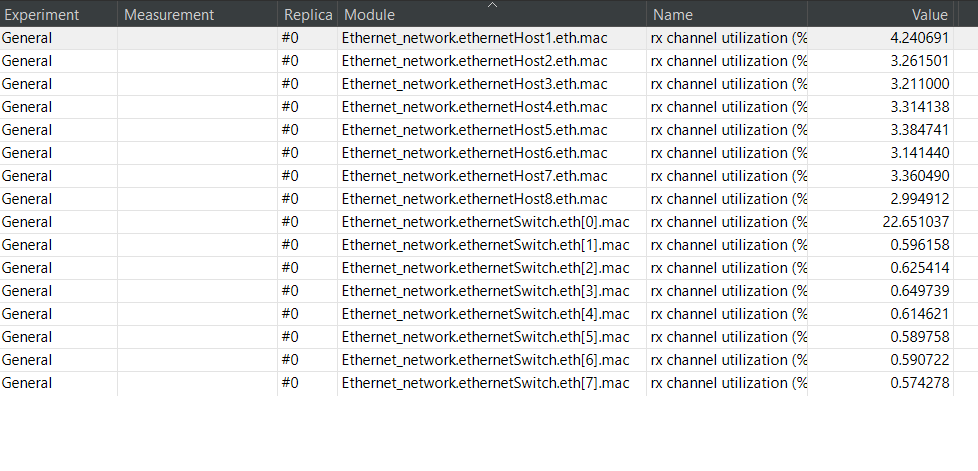
\includegraphics[width=0.7\textwidth]{output6.png}
            \caption{rx channel utilization(\%) for Q1 part 2}
        \end{figure}
        \begin{figure}[H]
            \centering
            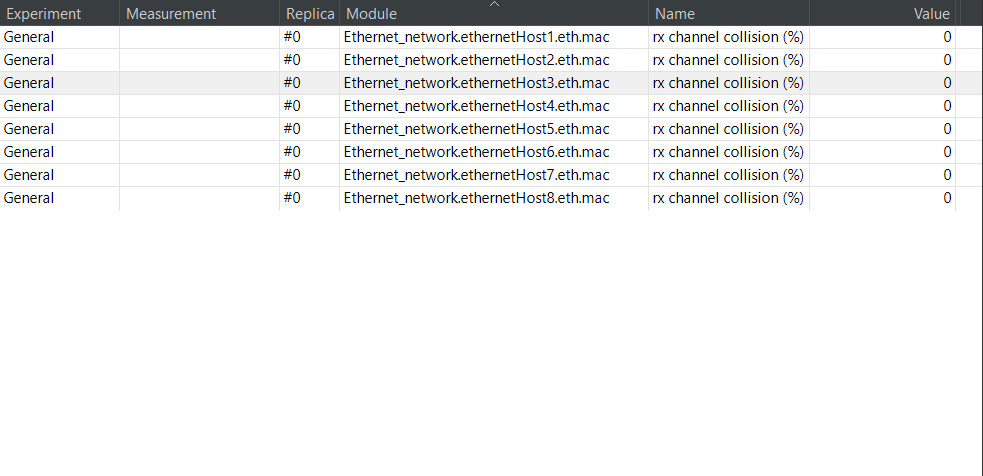
\includegraphics[width=0.7\textwidth]{output7.png}
            \caption{rx channel collision(\%) for Q1 part 2}
        \end{figure}
        \begin{figure}[H]
            \centering
            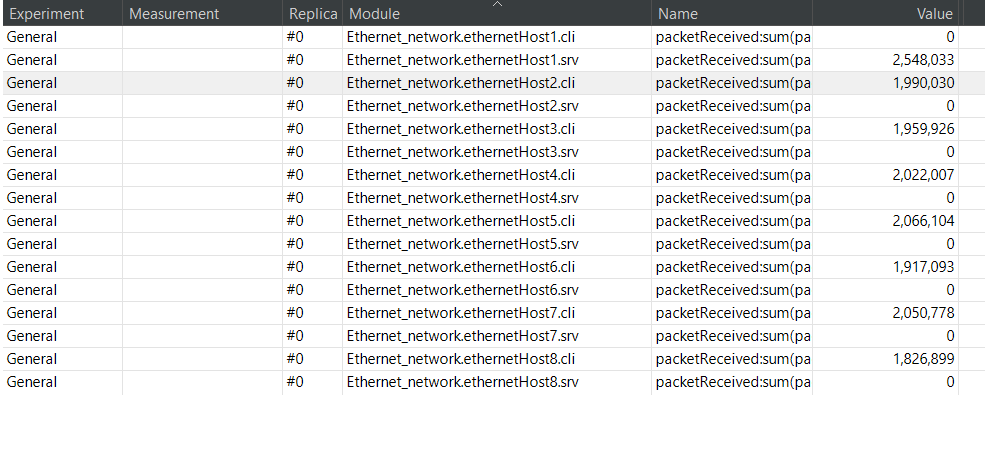
\includegraphics[width=0.7\textwidth]{output8.png}
            \caption{packetReceived:sum(packetBytes) for Q1 part 2}
        \end{figure}
        \begin{figure}[H]
            \centering
            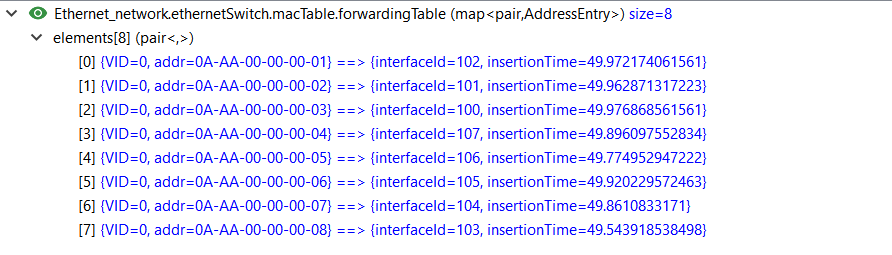
\includegraphics[width=0.6\textwidth]{output9.png}
            \caption{MAC address table for EthernetSwitch}
        \end{figure}
        \splitqsolve[\splitqsolve]
        so we can calculate the network throughput as $\frac{11766733\times 8\ bits}{50\ s} \simeq  1.88 Mbps$.so the network throughput is increased by 1 kbps. the collision rate using switch is 0\% because switch store the packets and send them when the channel is free but hub sends the packets to all hosts and if two hosts send packets at the same time the packets collide and the collision rate increases. so the switch is better than hub in terms of collision rate and network throughput.
    \end{qsolve}
\end{qsolve}
\subsection{part 3}
In this part we are going to simulate the network shown in Figure 3 (pay attention to distances depicted in the figure). This configuration has both \texttt{EthernetSwitch} and \texttt{EthernetHub}. We connect the vector of \texttt{EthernetHost} modules to the switch. To define the vector you can go to properties of one \texttt{EthernetHost} in the Design mode of your \texttt{.ned} file and enter the parameter \texttt{k} in front of the vector as shown in Figure 4. You should also add parameter \texttt{k} to your network definition in Source mode of \texttt{.ned} file like below:
\begin{verbatim}
    network MixedLAN
    {
        parameters:
            ...
            int k;
            ...
    }
    \end{verbatim}
    
    Then, in Source mode, you can easily connect all \texttt{k} hosts to the switch using a single \texttt{for} loop. Use \texttt{Eth10M} for all connections. We aim to conduct some experiments to determine the impact of packet size and traffic load on network throughput. To accomplish this, you must simulate the network across six scenarios (remember that \texttt{k} represents the number of hosts connected to the switch):
    
    \begin{itemize}
        \item scenario1: \texttt{reqLength=500B , k=8}
        \item scenario2: \texttt{reqLength=500B , k=20}
        \item scenario3: \texttt{reqLength=500B , k=100}
        \item scenario4: \texttt{reqLength=500B , k=200}
        \item scenario5: \texttt{reqLength=100B , k=8}
        \item scenario6: \texttt{reqLength=1400B , k=8}
    \end{itemize}
    
    The other settings in the \texttt{.ini} file are the same as in Part 1. After calculating the network throughput for each scenario, compare them. What is the impact of traffic load and packet size on network throughput? What is the ideal maximum throughput that can be achieved in this network? Why?
    
\begin{qsolve}
    \begin{qsolve}[]
        the network is shown in figure 13. to setup k hosts i used the code shown in figure 14 from .ned file. at last we set the reqLength and k in the .ini file.
        \begin{figure}[H]
            \centering
            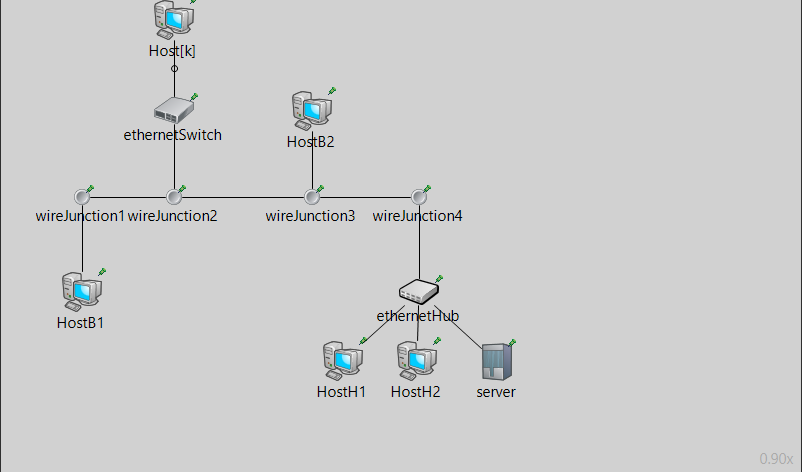
\includegraphics[width=0.8\textwidth]{Q1_3ned.png}
            \caption{network for Q1 part 3}
        \end{figure}
        \begin{figure}[H]
            \centering
            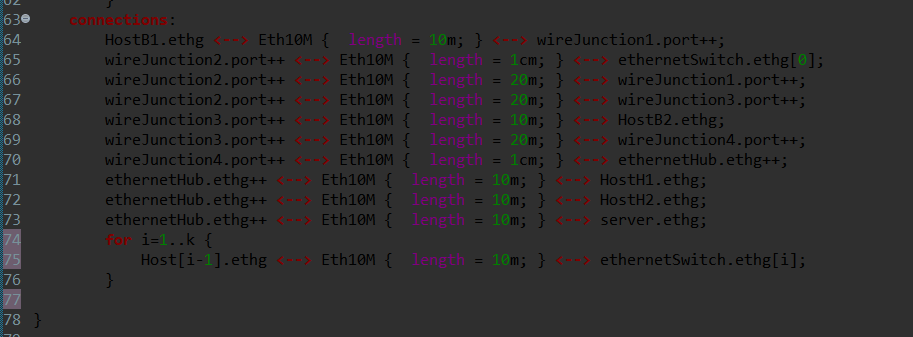
\includegraphics[width=0.8\textwidth]{Q1_3nedfor.png}
            \caption{setting up k hosts in ned file}
        \end{figure}
        \begin{figure}[H]
            \centering
            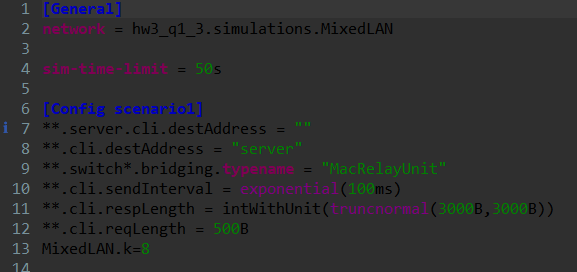
\includegraphics[width=0.8\textwidth]{Q1_3ini.png}
            \caption{ini file for Q1 part 3}
        \end{figure}
        \splitqsolve[\splitqsolve]
        by selecting each scenario in simulation menu we can get the outputs as below:
        \begin{figure}[H]
            \centering
            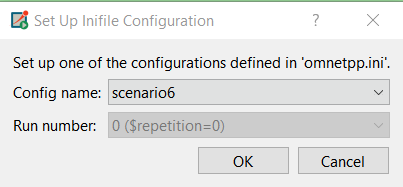
\includegraphics[width=0.45\textwidth]{output10.png}
            \caption{simulation menu}
        \end{figure}
        so the throughputs will be calculated as below:
        \begin{table}[H]
            \centering
            \begin{tabular}{|c|c|}
            \hline
             & Throughput \\
            \hline
            Scenario 1 &  3.39 Mbps\\
            \hline
            Scenario 2 &  6.77 Mbps\\
            \hline
            Scenario 3 &  9.54 Mbps\\
            \hline
            Scenario 4 &  9.7 Mbps\\
            \hline
            Scenario 5 &  3.53 Mbps\\
            \hline
            Scenario 6 &  3.02 Mbps\\
            \hline
            \end{tabular}
            \caption{Network throughput for different scenarios}
            \label{table:throughput}
        \end{table}
        the plot of this table is shown in figure 17. as we can see the network throughput increases by increasing the number of hosts but in a fixed number of hosts if the packet size increases the network throughput decreases. the ideal maximum throughput that can be achieved in this network is 10 Mbps because the minimum throuput of channels is 10 Mbps and throughput cant reach a number higher than that.
        \begin{figure}[H]
            \centering
            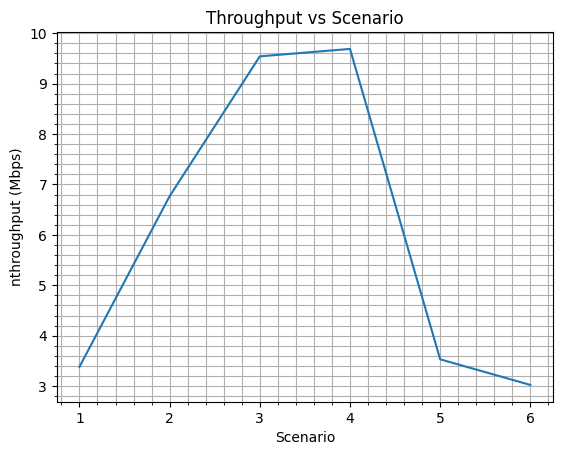
\includegraphics[width=0.6\textwidth]{output11.png}
            \caption{Network throughput for different scenarios}
        \end{figure}
    \end{qsolve}
\end{qsolve}